\documentclass[12pt]{article}


\begin{document}
Notre projet dispose de plusieurs formes qui sont utilisées pour le rendu des scènes. Les deux formes les plus utilisées sont le plan et la sphère. Nous avons aussi implémenté les parallélépipèdes, les prismes, les pyramides, ...
Une forme plus technique que les autres que nous avons implémenté est l'icosphère.
\subsubsection{Définition d'une icosphère}
L'Icosphère est une sphère construite avec des triangles et un nombre de subdivisions donné. La \figurename \ref{fig:image_subdiv} montre des icosphères avec des nombres de subdivisions différents.

\subsubsection{Construction d'une icosphère}
En partant de 20 triangles positionnés d'une certaine façon, nous pouvons calculer des subdivisions.
Chaque subdivision multiplie le nombre de triangle de l'icosphère par 4 en divisant chaque triangle existant en 4 nouveaux.
L'icosphère se rapproche alors, après chaque subdivision, d'une sphère parfaite.
L'image \ref{fig:image_subdiv} ci-dessous montre la différence entre des icosphères de subdivision 1, 3 et 5.

\begin{figure}[ht]
  \begin{center}
    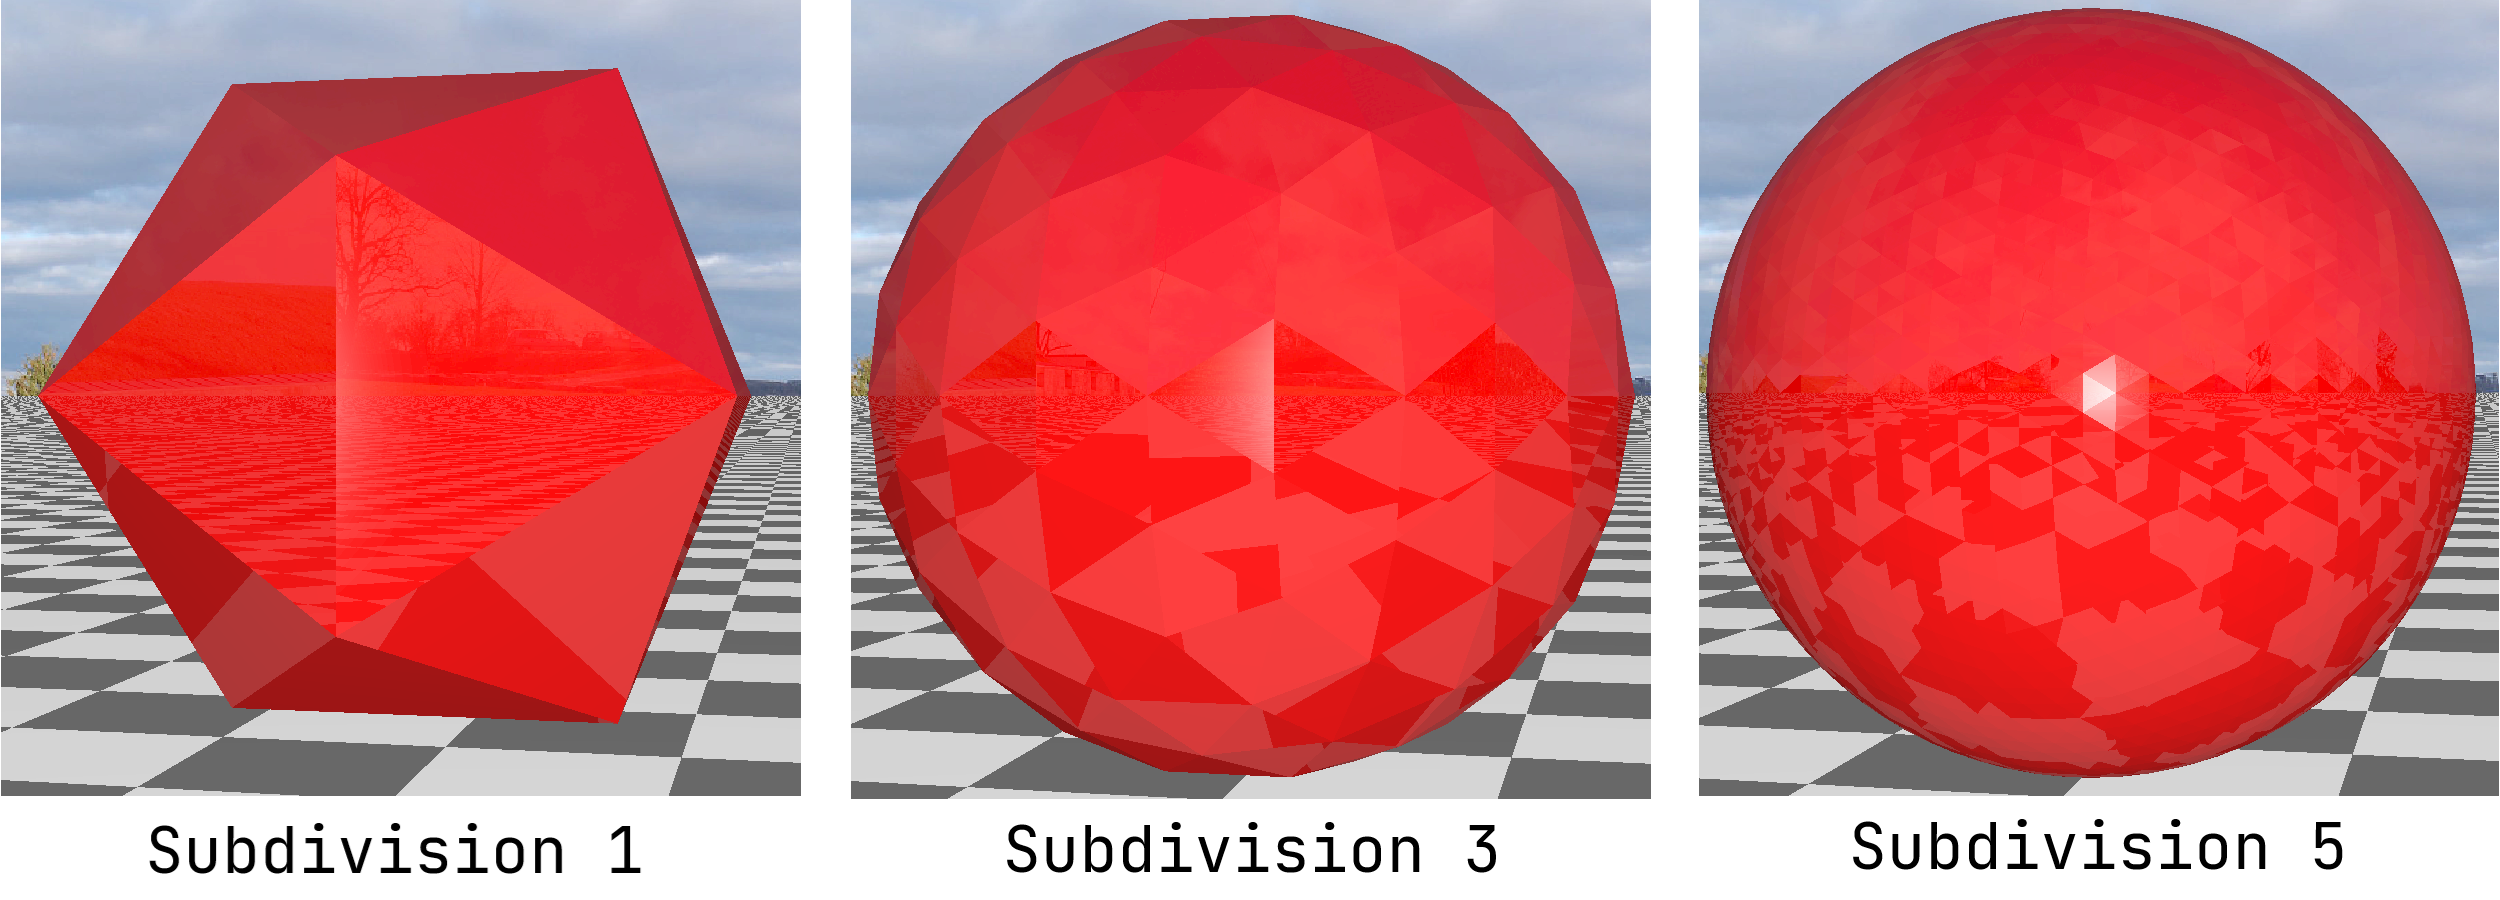
\includegraphics[width=0.7\textwidth]{./img/formes/subdivicosp.png} 
  \caption{Plusieurs icosphères de subdivisions différentes}
  \label{fig:image_subdiv}
\end{center}
\end{figure}
\FloatBarrier



\end{document}
